\section{Amdahl's law}

When analyzing the potential improvement in execution time provided by parallel
threads of execution, the runtime of the problem under consideration has to be
separated in two categories: one that can be executed in parallel and one that
has to be serialized.  Given a proportion $p$ between the two, the total
execution time $T$ is:

\begin{align*}
    T = (1 - p)T + pT \\
\end{align*}

The serial portion cannot by definition be accelerated with additional threads
of execution.  Any speedup factor $s$ is applied only to the $p$ factor, such
that the new execution time $T(s)$ is:

\begin{align*}
    T(s) &=  (1 - p)T + \frac{p}{s}T \\
         &= (1 - p   + \frac{p}{s})T \\
\end{align*}

Thus, the speedup $S$ for any process is:

\begin{align*}
    S &= \frac{T}{T(s)} \\
      &= \frac{T}{(1 - p + \frac{p}{s})T} \\
      &= \frac{1}{ 1 - p + \frac{p}{s}} \\
\end{align*}

This general formulation is \textit{Amdahl's law} for the latency speedup of an
improvement to a system as a function of the proportion of that system to which
the improvement applies\footnotemark.  Figure \ref{fig:conc:amdahl} shows the
plot of this relation for different values of $p$ and $s$.  It is evident that,
at any level of parallelism, even a small portion of serial work is a
significant bottleneck.  The inability to use the additional processing power is
more pronounced the higher the processor count, and eventually any amount of
serial work becomes a limitation, a vertical asymptote:

\begin{align*}
    S &= \frac{1}{1 - p + \frac{p}{s}} \\
    \lim\limits_{s \to \infty} S &= \frac{1}{1 - p} \\
\end{align*}

\footnotetext{
    This general definition applies to any kind of system, including serial
    processes.  Seen in another way, Amdahl's law states the impact of improving
    one of the phases of a process given the proportion of the total execution
    time it represents.}

\begin{figure}[ht]
    \centering
    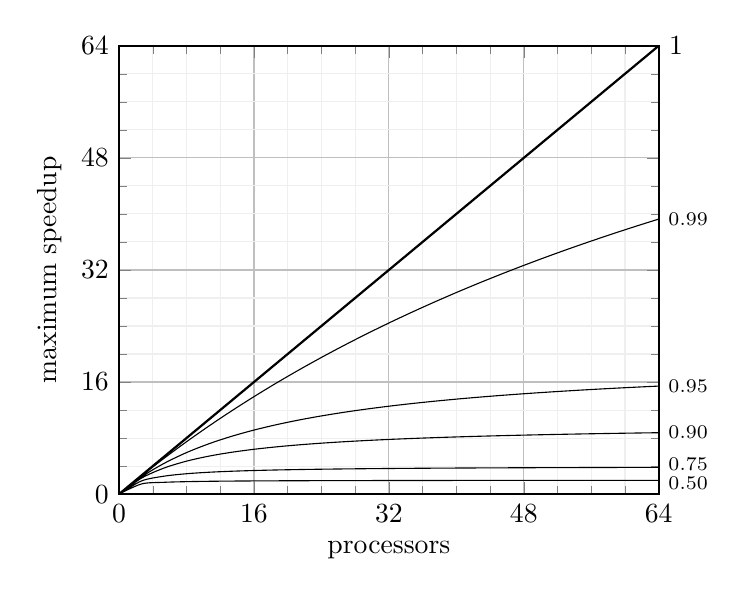
\begin{tikzpicture}
        \begin{axis}[
            domain = 0:64, thick, smooth, clip = false,
            xlabel = processors, ylabel = maximum speedup,
            xmin = 0, xmax = 64, ymin = 0, ymax = 64,
            xtick distance = 16, ytick distance = 16,
            minor tick num = 3,
            grid = both,
            major grid style = {lightgray},
            minor grid style = {lightgray!25},
        ]
            \def\p#1#2{
                plot[domain = 0:64] (\x, {1 / (1 - #1 + (#1 / \x))})
                node[right, black, yshift = #2] {#1}
            }
            \draw[black] plot[domain = 0:64] (\x, \x) node[right] {1};
            \draw[black, thin, font = \scriptsize]
                \p{0.99}{0}
                \p{0.95}{0}
                \p{0.90}{0}
                \p{0.75}{+0.1em}
                \p{0.50}{-0.1em};
        \end{axis}
    \end{tikzpicture}
    \caption{Amdahl's law applied to parallel processors}
    \label{fig:conc:amdahl}
\end{figure}

The fundamental rule on which this law is predicated is very simple: a program
will never be faster than its serial portion, no matter how many resources are
added.  A program that is 10\% serial has a maximum speedup of 10 ($\frac{1}{1 -
0.1} = 10$), as the 10\% will never be affected by the addition of resources.
I.e. the theoretical maximum speedup of a process is always limited by its
serial portion.
